\documentclass[aspectratio=169]{beamer}

\usepackage[T2A]{fontenc}
\usepackage[utf8]{inputenc}
\usepackage[english, russian]{babel}
\usepackage{amsfonts}
\usepackage{amsmath}
\usepackage{multirow}
\usepackage{multicol}
\usepackage{tabularx}
\usepackage{hhline}
\usepackage{titlesec}

\usepackage{graphicx}
\graphicspath{{}}
\DeclareGraphicsExtensions{.pdf,.png,.jpg}

\newcommand{\sectionbreak}{\clearpage}

\usepackage{xltxtra}
\usepackage[main=russian,english]{babel}


\title{AVL деревья}
\institute[СГУ им. Чернышевского]{Саратовский Государственный Университет им. Чернышевского}
\author{Еремеев Тимур}
\data{2022}

\begin{document}

    % Титульный слайд
    \frame{\titlepage}
    
    % Оглавление
    %\frame{\tableofcontents}

    % Введение
    % второй слайд
    \begin{frame}
    \section{Введение}
    
    AVL"=дерево "--- сбалансированное по высоте бинарное дерево поиска:
    для каждой его вершины высота её двух поддеревьев различается не более чем на 1.

    AVL "--- аббревиатура, образованная первыми буквами создателей
    (советских учёных) Г. М. Адельсон-Вельского и Е. М. Ландиса.
\end{frame}
    
    % Общие св-ва - начало
    % третий слайд
    \begin{frame}
    \frametitle{Общие св-ва}
    
    В AVL"=дереве высоты $h$ имеется не меньше $F_h$ узлов, где $F_h$ "--- число Фибоначчи.
    Поскольку $F_n = \frac{(\frac{1 + \sqrt{5}}{2})^n - (\frac{1 - \sqrt{5}}{2})^n}{\sqrt{5}} =
    \frac{\phi^n - (-\phi)^{-n}}{\phi - (-\phi)^{-1}}$,
    где $\frac{\phi^n - (-\phi)^{-n}}{\phi - (-\phi)^{-1}}$ "--- золотое сечение,
    то имеем оценку высоты AVL-дерева $h = Q(\lg(n))$,
    где $n$ "--- число узлов. Следует помнить, что $Q(\lg(n))$ "--- мажоранта,
    и её можно использовать только для оценки
    (Например, если в дереве только два узла, значит в дереве два уровня,
    хотя $\lg(2) = 1$. Для точной оценки глубины дерева следует использовать пользовательскую программу.
\end{frame}

    % четвёртый слайд
    \begin{frame}
    %листинг
\end{frame}

    % пятый слайд
    \begin{frame}
    Тип Дерева можно описать так:

    % ещё один листинг
\end{frame}
    % Общие св-ва - конец

    % Балансировка - начало
    % шестой слайд
    \begin{frame}
    \section{Балансировка}

    Относительно AVL"=дерева балансировкой вершины называется операция,
    которая в случае разницы высот левого и правого поддеревьев $= 2$,
    изменяет связи предок-потомок в поддереве данной вершины так,
    что разница становится $ \leqslant 1$, иначе ничего не меняет.
    Указанный результат получается вращениями поддерева данной вершины.
    
\end{frame}

    % седьмой слайд
    \begin{frame}
    Используется 4 типа вращений:

    \frametitle{Малое левое вращение}

    %картинка 1
    \begin{figure}[ht]
        \includegraphics[width = \textwidth]{../../images/1.pdf}
        
        \caption{Схематическое изображение малого левого вращения}    
    \end{figure}

    Данное вращение используется тогда,
    когда (высота $b$"=поддерева; $L$ "--- высота )
    $= 2$ и высота $С \leqslant$ высота $R$.

\end{frame}

    % восьмой слайд
    \begin{frame}
    \frametitle{Большое левое вращение}

    %картинка 2
    \begin{figure}[ht]
    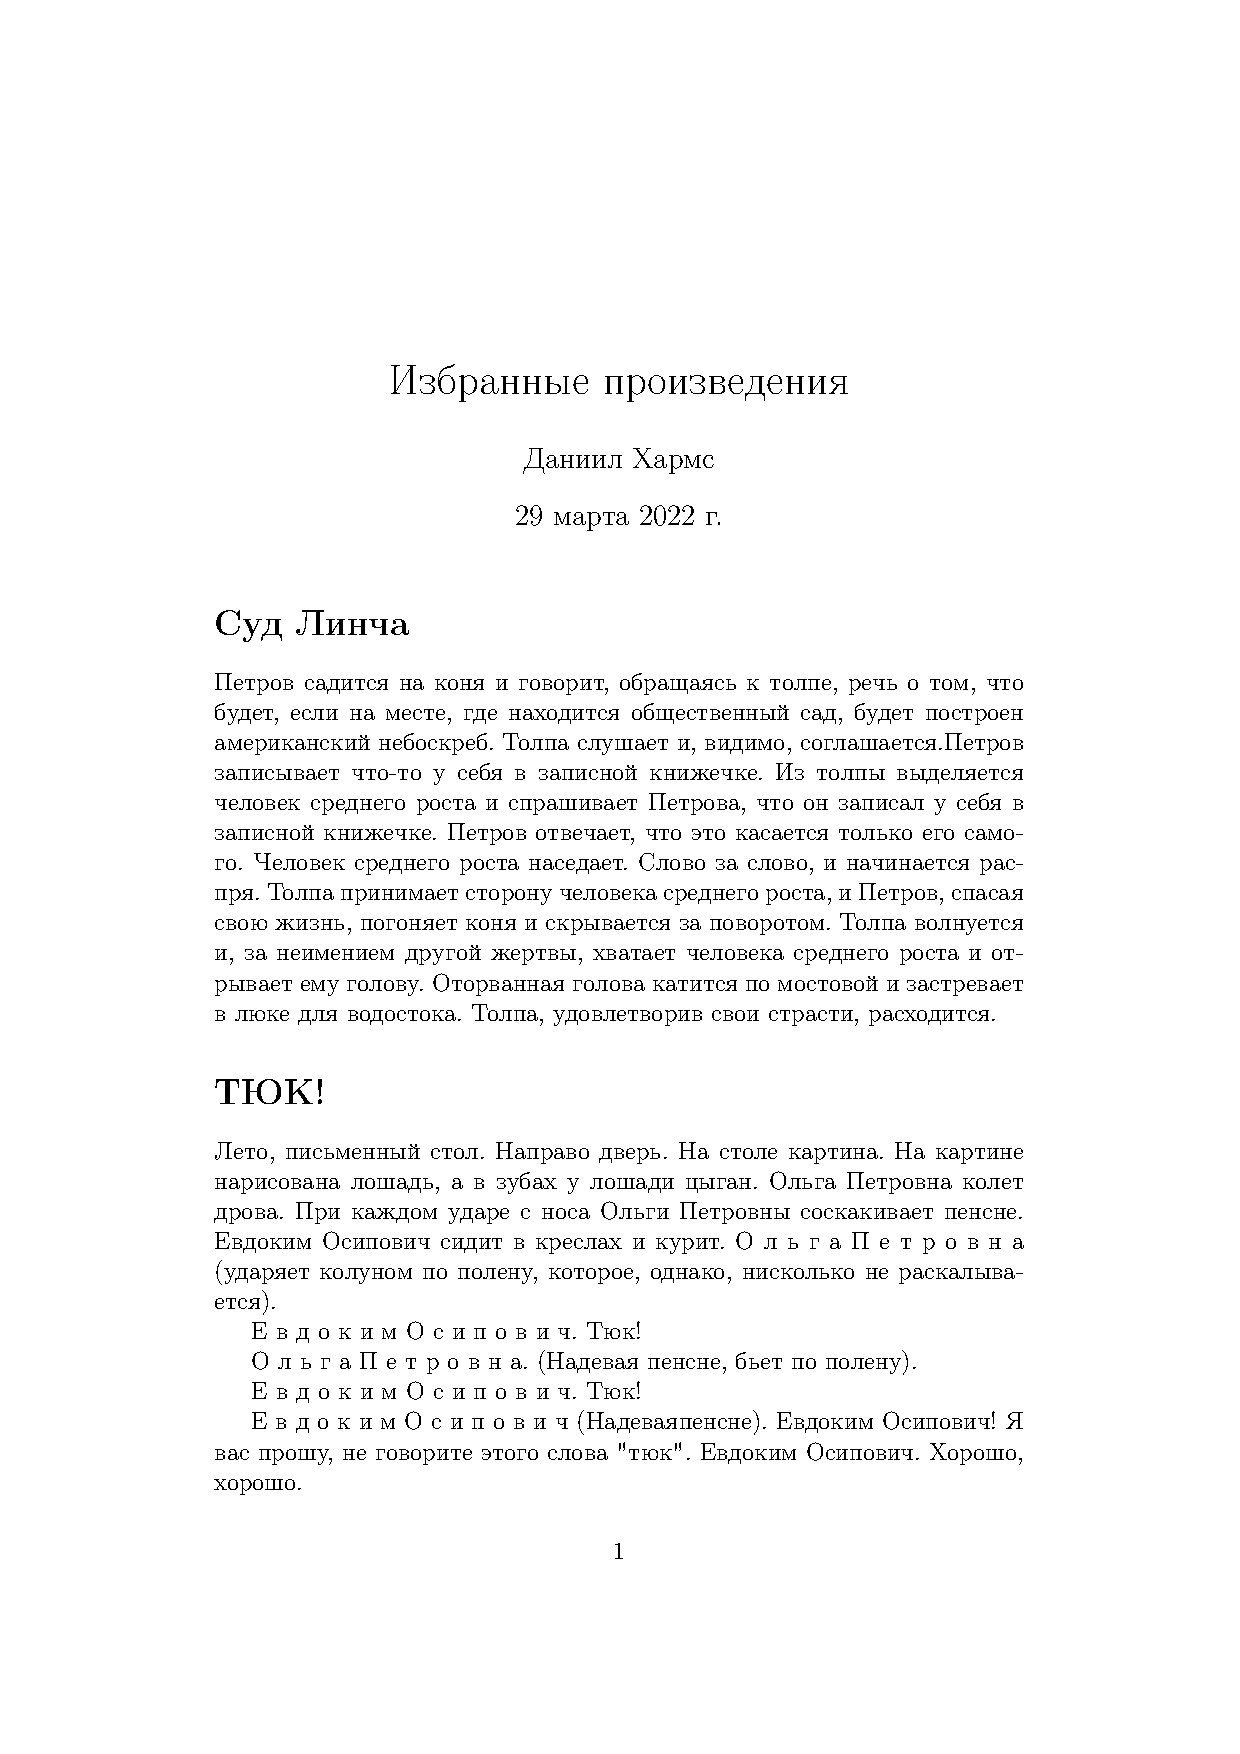
\includegraphics[width = \textwidth]{../imagen/2.gif}

    \caption{Схематическое изображение большого левого вращения}
    \end{figure}

    Данное вращение используется тогда,
    когда (высота $b$"=поддерева; $L$ "--- высота)
    $= 2$ и высота $c$"=поддерева $>$ высота $R$.
\end{frame}

    % девятый слайд
    \begin{frame}
    \subsection*{Малое правое вращение}

    %картинка 3
    \begin{figure}[ht]
        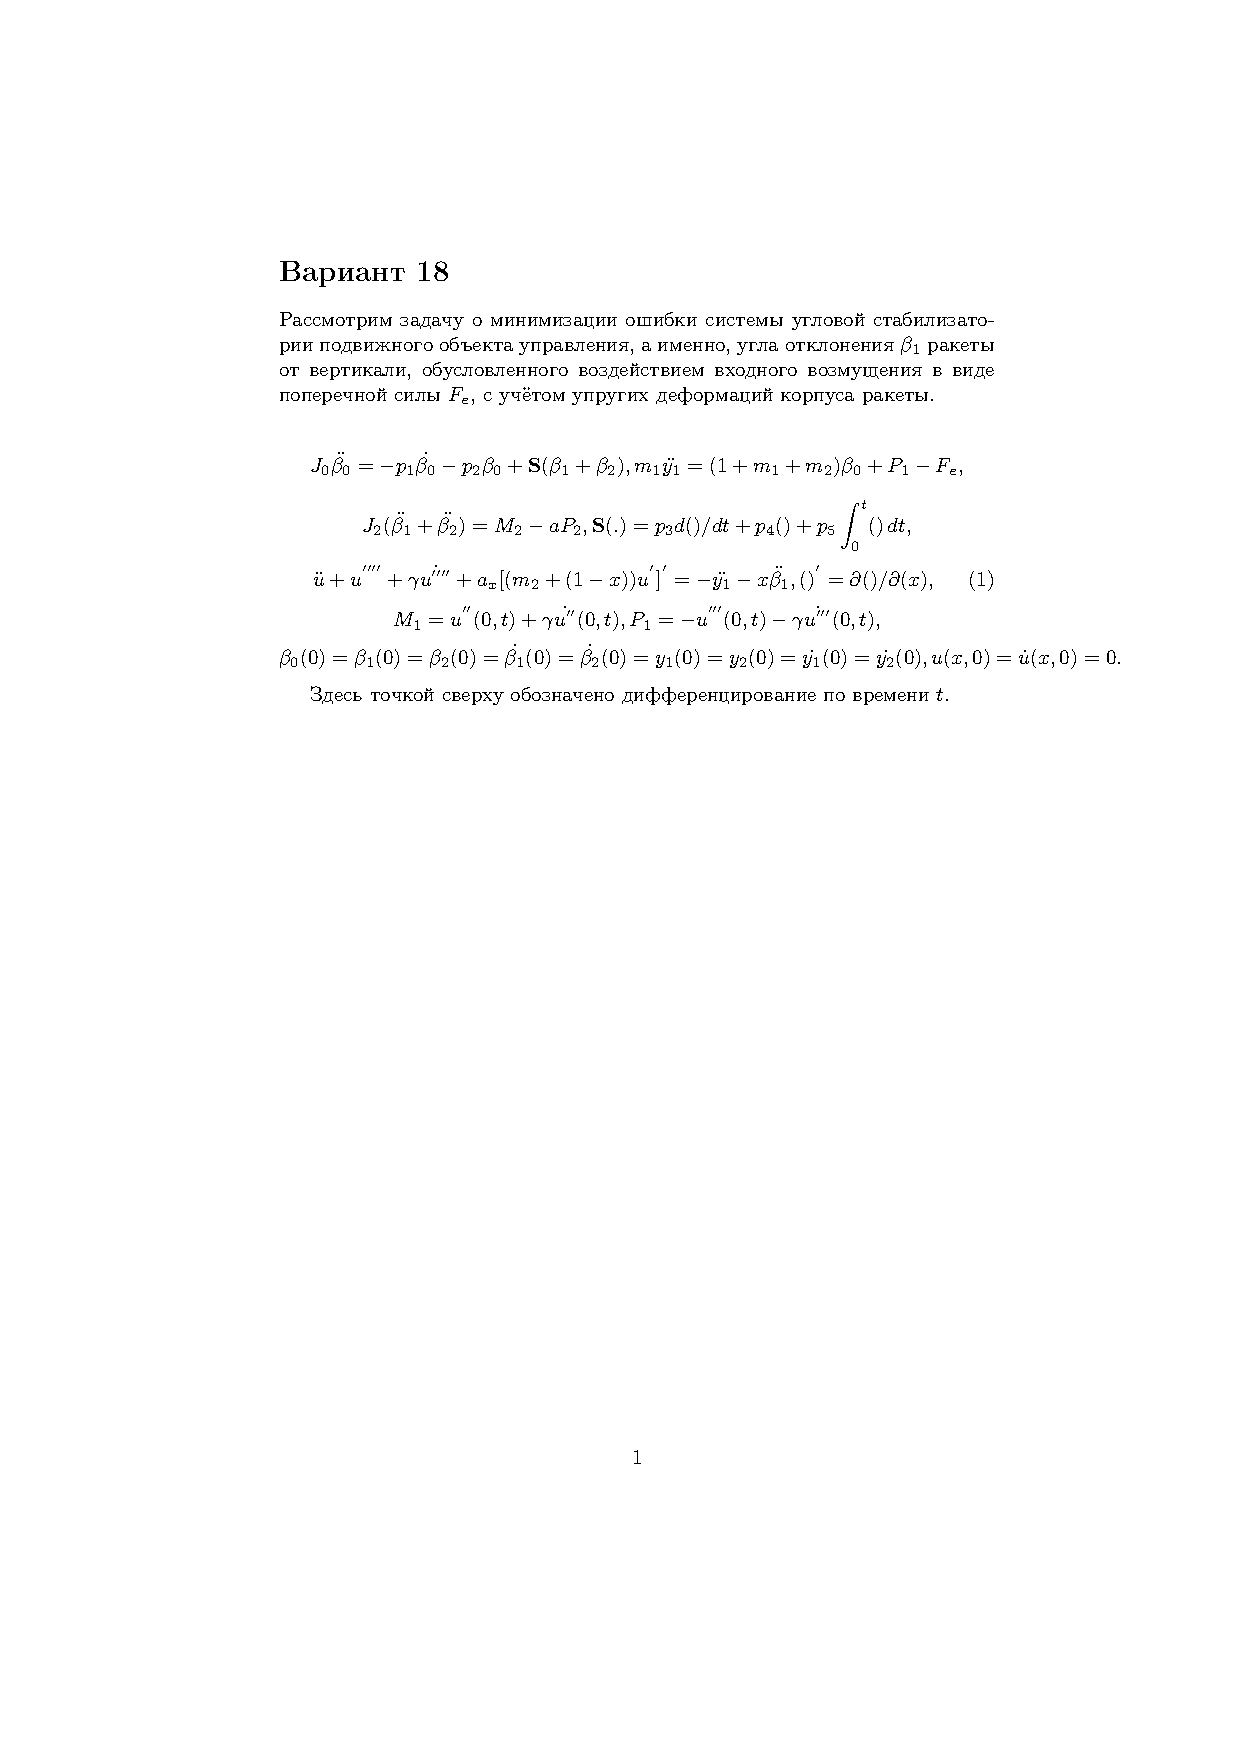
\includegraphics[width = \textwidth]{3.gif}
        
        \caption{Схематическое изображение малого правого вращения}
    \end{figure}

    Данное вращение используется тогда,
    когда (высота $b$"=поддерева "--- высота $R$)
    $= 2$ и высота $С \leqslant $ высоты $L$.
\end{frame}
    
    % десятый слайд
    \begin{frame}
    \frametitle{Большое правое вращение}

    %картинка 4
    \begin{figure}[ht]
        \includegraphics[width = \textwidth]{../../images/4.pdf}
        
        \caption{Схематическое изображение большого правого вращения}

    \end{figure}

    Данное вращение используется тогда, когда (высота $b$"=поддерева; $R$ "--- высота)
    $= 2$ ивысота $c$"=поддерева $ > $ высота $L$.
    В каждом случае достаточно просто доказать то, 
    что операция приводит к нужному результату и
    что полная высота уменьшается не более чем на $1$ и не может увеличиться.
    Из-за условия сбалансированности высота дерева $O(\lg(N))$,
    где $N$ "--- количество вершин, поэтому добавление элемента требует $Q(\lg(N))$ операций.
\end{frame}
    % Балансировка - конец

    % Алгоритм добавления вешины - начало
    % одиннадцатый слайд
    \begin{frame}

    \frametitle{Алгоритм добавления вершины}

    Показатель сбалансированности в дальнейшем будем интерпретировать
    как разность между высотой левого и правого поддерева,
    а алгоритм будет основаться на типе TAVLTree, описанном выше.
    Непосредственно при вставке (листу) присваивается нулевой баланс.
    Процесс включения вершины состоит из трех частей:

    \begin{enumerate}
        \item Прохода по пути поиска, пока не убедимся, что ключа в дереве нет.
        \item Включения новой вершины в дерево и определения результирующих показателей балансировки.
        \item "Отступления" назад по пути поиска и проверки в каждой вершине показателя сбалансированности.
        Если необходимо - балансировка
    \end{enumerate}
\end{frame}
        
    % двенадцатый слайд
    \begin{frame}
    Расширим список параметров обычной процедуры вставки параметром-переменной flag,
    означающим, что высота дерева увеличилась.
    Предположим, что процесс из левой ветви возвращается к родителю (рекурсия идет назад),
    тогда возможны три случая:
    {$h_1$ "--- высота левого поддерева, $h_r$- высота правого поддерева}
    Включение вершины в левое поддерево приведет к

    \begin{enumerate}
        \item $h_1 < h_r$: выровняется $h_1 = h_r$. Ничего делать не нужно.
        \item $h_1 = h_r$: теперь левое поддерево будет больше на единицу,
        но балансировка пока не требуется.
        \item $h_1 > h_r$: теперь $h_1 - h_r = 2$, "--- требуется балансировка.
    \end{enumerate}
\end{frame}
    
    % тринадцатый слайд
    \begin{frame}
    %листинг
\end{frame}
    
    % четырнадцатый слайд
    \begin{frame}
    %листинг
\end{frame}
    % Алгоритм добавления вершин - конец

    % Алгоритм удаления вершины - начало
    % пятнадцатый слайд
    \begin{frame}
    \frametitle{Алгоритм удаления вершин}

    Для простоты опишем рекурсивный алгоритм удаления.
    Если вершина "--- лист, то удалим её и вызовем балансировку всех её предков в порядке от родителя к корню.
    Иначе найдём самую близкую по значению вершину в поддереве наибольшей высоты (правом или левом) и переместим её на место удаляемой вершины,
    при этом вызвав процедуру её удаления.

\end{frame}


    % шестнадцатый слайд
    \begin{frame}
    Докажем, что данный алгоритм сохраняет балансировку.
    Для этого докажем по индукции по высоте дерева,
    что после удаления некоторой вершины из дерева и
    последующей балансировки высота дерева уменьшается не более, чем на 1.
    База индукции: Для листа очевидно верно.
    Шаг индукции: Либо условие балансированности в корне (после удаления корень может изменится) не нарушилось,
    тогда высота данного дерева не изменилась,
    либо уменьшилось строго меньшее из поддеревьев $ $
    высота до балансировки не изменилась $ $
    после уменьшится не более чем на 1.
    
\end{frame}

    % семнадцатыый слайд
    \begin{frame}
    Очевидно, в результате указанных действий процедура удаления вызывается не более 3 раз,
    так как у вершины, удаляемой по 2-му вызову, нет одного из поддеревьев.
    Но поиск ближайшего каждый раз требует $O(N)$ операций,
    отсюда видна очевидная оптимизация:
    поиск ближайшей вершины производится по краю поддерева.
    Отсюда количество действий $O(\lg(N))$.

\end{frame}
    % Алгоритм удаления вершины - конец

    % Расстановка балансов при удалении - начало
    % восемнадцатый слайд
    \begin{frame}
    \frametitle{Расстановка балансов при удалении}

    Как уже говорилось, если удаляемая вершина"="лист, то она удаляется,
    и обратный обход дерева происходит от родителя удалённого листа.
    Если не лист "--- ей находится «замена», и обратный обход дерева происходит от родителя «замены».
    Непосредственно после удаления элемента "--- «замена» получает баланс удаляемого узла.

\end{frame}

    % девятнадцатый слайд
    \begin{frame}
    При обратном обходе: если при переходе к родителю пришли слева "--- баланс увеличивается на $1$,
    если же пришли справа "--- уменьшается на $1$.
\end{frame}

    % двадцатый слайд
    \begin{frame}
    
    Это делается до тех пор, пока при изменении баланса он не станет равным $-1$ или $1$
    (обратите внимание на различие с вставкой элемента!):
    в данном случае такое изменение баланса будет гласить о неизменной дельта-высоте поддеревьев.
    Повороты происходят по тем же правилам, что и при вставке.

\end{frame}
    % Расстановка балансов при удалении - конец

    % Расстановка при одинарном повороте - начало
    % двадцать первый слайд
    \begin{frame}
    \frametitle{Расстановка при одинарном повороте}

    Обозначим:

    «Current» "--- узел, баланс которого равен $-2$ или $2$:
    то есть тот, который нужно повернуть (на схеме - элемент a)

    «Pivot» "--- ось вращения. $+2$: левый сын Current'а, $-2$: правый сын Current'а (на схеме "--- элемент $b$)

    Если поворот осуществляется при вставке элемента, то баланс Pivot'а равен либо $1$, либо $-1$.
    В таком случае после поворота балансы обоих устанавливаются равными $0$.

    При удалении всё иначе: баланс Pivot'а может стать равным $0$ (в этом легко убедиться).

\end{frame}

    % двадцать второй слайд
    \begin{frame}

    Приведём сводную таблицу зависимости финальных балансов от направления поворота и исходного баланса узла Pivot:

    \begin{table*}[ht]
        \centering
    
        \begin{tabular}{|c|c|c|c|}
            \hline
            Направление поворота & Old Pivot Balance & New Current Balance & New Pivot Balance \\
            \hline
                Левый или правый &   $-1$ или $+1$   &         $0$         &        $0$        \\
            \hline
                          Правый &        $0$        &         $-1$        &        $+1$       \\
            \hline
                           Левый &        $0$        &         $+1$        &        $-1$       \\
            \hline
        \end{tabular}
    
    \end{table*}

\end{frame}
    % Расстановка при одинарном повороте - конец

    % Расстановка балансов при двойном повороте - начало
    % двадцать третий слайд
    \begin{frame}
    \frametitle{Расстановка балансов при двойном повороте}

    Pivot и Current "--- те же самые, но добавляется третий участник поворота.
    Обозначим его за «Bottom»: это (при двойном правом повороте) левый сын Pivot'а,
    а при двойном левом "--- правый сын Pivot'а.

    При данном повороте "--- Bottom в результате всегда приобретает баланс $0$,
    но от его исходного баланса зависит расстановка балансов для Pivot и Current.

\end{frame}

    % двадцать четвёртый слайд
    \begin{frame}
    
    Приведём сводную таблицу зависимости финальных балансов от направления поворота и исходного баланса узла Bottom:

    \begin{table*}[ht]
        \centering
    
        \begin{tabular}{|c|c|c|c|}
            \hline
            Направление поворота & Old Botom Balance & New Current Balance & New Pivot Balance \\
            \hline
                Левый или правый &        $0$        &         $0$         &        $0$        \\
            \hline
                          Правый &        $+1$       &         $0$         &        $-1$       \\
            \hline
                          Правый &        $-1$       &         $+1$        &        $0$       \\
            \hline
                           Левый &        $+1$       &         $-1$        &        $0$       \\
            \hline
                           Левый &        $-1$       &         $0$         &        $+1$       \\
            \hline
        \end{tabular}
    
    \end{table*}

\end{frame}
    % Расстановка балансов при двойном повороте - конец

    % Оценка эффективности
    % двадцать пятый слайд
    Г.М.Адельсон-Вельский и Е.М.Ландис доказали теорему,
согласно которой высота AVL"=дерева с $N$ внутренними вершинами заключена между $log2(N+1)$ и $1.4404*log2(N+2)-0.328$,
то есть высота AVL"=дерева никогда не превысит высоту идеально сбалансированного дерева более,чем на $45\%$.
Для больших N имеет место оценка $1.04*log2(N)$.
Таким образом, выполнение основных операций $1"=3$ требует порядка $log2(N)$ сравнений.
Экспериментально выяснено, что одна балансировка приходится на каждые два включения и на каждые пять исключений.

    % Список источников
    % двадцать шестой слайд
    \begin{frame}
    \frametitle{Источнки}

    \begin{enumerate}
    \item Особенность изучения сбалансированных деревьев бинарного поиска
    https://elibrary.ru/item.asp?id=41829778

    \item Сравнительный анализ производительности функций, связанных с AVL-деревьями
    https://elibrary.ru/item.asp?id=32881485

    \item Хранение и обработка информации с помощью иерархических cтруктур данных
    https://elibrary.ru/item.asp?id=29275683

    \end{enumerate}

\end{frame}

\end{document}